Thesis thoughts:

Intro/background: 
- QCD
- Hadronic Particle Production
	- Jets in Heavy Ion Collisions
- Relativistic Heavy Ion Collisions
	- Transverse Energy in Heavy Ion Collisions
	- Interplay of Hard and Soft Processes in Heavy Ion Collisions
- Monte Carlo Generators

- QCD
	- QCD Langragian 
	- Feynman Rules and Running of the Coupling Constant
	- Perturbative QCD
	    - Factorization Theorem
	    - Deep Inelastic Scattering
	    - Parton Distribution Functions
	- Parton showers
	    - Initial State Radiation
	    - Final State Radiation
	    - Jet Algorithms

- QGP
	- Existence of Quark Gluon Plasma
	- QCD Phase Diagram - not priority 
	- Lattice QCD/EOS - not priority
	- Relativistic Heavy Ion Collisions
	    - Initial State and Bjorken Energy Density
	    - Glauber model
	    - Binary Scaling

- Modeling of Heavy Ion Collisions
	- Relavistic Heavy Ion Collision Phenomenology
	    - Initial State
	    - Thermalization
	    - Hydrodynamic Evolution
	    - Hadronization
	    - Freeze-out
	- Monte Carlo Generators and Models
		- Pythia
			- references - TH1, 98, 99, 102, 103, 201, 202
		- Herwig
			- references - TH1, 96, 97, 107, 203, 204, 205
		- HIJING
		- AMPT
		- EPOS4

- Interplay of Hard and Soft Processes in Heavy Ion Collisions - 1-2 pages
	- Different energy scales 
	- Brians slides on hard and soft processes
	- 2 to 3 jet cross sections 
	- ATLAS/CMS/STAR results 


pQCD
factorization:
factorization - short and long distance behavior are separated
cross section for hard scattering in hadron hadron collision 
factorization scale, energies (Q) above mu_f are short range and energies below are long range
fragmentation function D describes the non perturbative parts of hadronic processes including partons fragmenting into hadrons 
F are parton distribution functions - PDF are distributions of number density of a given parton within the hadron carrying a fraction f of the hadrons momentum 
PDF is not perturbatively calculable instead found from experiment in DIS 
separation of scales allows neglect of quantum mechanical interference between the different calculation components 
factorization holds for DIS and e+e- collisions and Drell Yan but is only approximate in other QCD systems 
wavelength of virtual photon has to be small and resolving structure of object must be fine
DIS:
point like consistuents of hadrons comes from measurements of deep inelastic electron-proton scattering
highly virtual photon exchange between electron and hadron, shattering the hadron
Bjorken-x - the fraction of the nucleons momentum carried by the struck quark in the infinite momentum frame
DIS has conditions of deep: Q^2 >> M^2 (mass of nucleon) and inelastic: W^2 >> M^2 recoil of system is much larger than mass of nucleon, wavelength of virtual photon must be small 
bjorken x equations and scaling 
differential cross section for DIS 
structure function equations 
F are nucleon structure functions 
very weak dependence of Q^2 at fixed x, bjorken scaling, scattering in DIS occurs from point-like constituents in nucleon
higher order corrections are included the structure function is modified - parton that comes out can undergo splittings before the hard scattering with the virtual photon
PDFs:
the fundamental description of collinear hadronic structure in terms of partonic constituents 
PDFs subject to conservation laws for charge, flavor and momentum requiring that the total charge and momentum of the proton is conserved and two up one down and no net strangeness or other heavy quark 
the conservation laws help to eliminate extra degrees of freedom in the structure functions that are inputs into the cross section 
Callon-gross relation reflects spin 1/2 nature of the partons 
DGLAP equations govern the evolution in Q^2 and alpha s of PDFs
splitting functions, probability of parton b splitting into pair of partons, including parton a with fraction of parent’s momentum x
collinear factorization (MS bar renormalization scheme) introduces factorization scale mu_f that separates the hard emissions from the soft emissions in the PDFs
PDF fitting is done by parameterization in terms of higher order polynomials in x at some initial scale Q0^2 and then they are evolved using the DGLAP evolution where other data is available, then PDFs are used as input to perturbative calculations of cross-sections for different observables 

If gluon is required to be separated from quark anti-quark hard scattering in three jet event then cross section for process is proportional to alpha_s * cross section for two jet process.

DIS notes:
wavelength of virtual photon has to be small and resolving structure of object must be fine
cross section for scattering of electron off a target of mass m charge e and magnetic moment e/2M
generalized form in terms of many structure functions using “ingredients” g_munu *p * q
“W are functions of scalars built from variables at the vertex”
use current conservation to eliminate two of the structure functions and left with two lorentz invariant structure functions at the vertex 
Write everything in terms of bjorken x and y
at high Q^2/bjroken scaling find that F1 and F2 have a relationship and it only depends on Q^2/2mnu
Here is were the callan Gross relation reflects the spin 1/2 nature of the partons 
characteristic interaction time between the quark and virtual photon must be small in comparison to the interaction between the partisan in protons 
F2(x) can be solved for from cross section measurements
conservation of quark flavors also inform structure functions (sum rules) 

Intro1:
- QCD
	- QCD Langragian 
		- Feynman Rules
		- QCD Beta Function
		- Lattice QCD
	- Confinement and Asymptotic Freedom
	- QCD Factorization and Parton Model
- Nuclear Structure (?)
- Hadronic Particle Production
	- Fragmentation Functions
	- Parton Showers
	- Models of Hadronization
- Relativistic Heavy Ion Collisions
	- Collision Centrality and Geometry
	- QGP
- Monte Carlo Generators

Intro2: 
- Standard model
	- QCD
- Heavy Ion Collisions
- Jets and Underlying Event
	- Jets in Heavy Ion Collisions 
	- Jet Background Subtraction

Intro3: 
- QCD
	- Asymptotic Freedom and Confinement
	- Particle Content
	- Factorization and DIS
	- Parton Distribution Functions
	- QCD Jets
- QCD at high densities and high temperatures
	- Geometry of nuclear collisions

Intro4: 
- Standard Model
- QCD
- Factorization and Parton Distribution Function
- Small-x and Gloun Saturation
- Jets
- QGP
- Phenomenology of the QGP
- Collectivity 

Intro5: 
- QCD
- Perturbative QCD 
	- Factorization and parton model
	- Fragmentation functions
	- Jets
- QGP
	- QCD Phases
	- Lattice thermodynamics
	- Relativistic heavy ion collisions
	- Hydrodynamics 
	- Collectivity
- Hard Processes in Heavy Ion Collisions
	- Glauber Model
	- Nuclear PDF
	- Parton energy loss and jet quenching



HIJING is a high-energy heavy ion and proton-proton collision event generator that uses a glauber model of the nuclei geometry and perturbative QCD to model hard scatterings as minijets including multi- parton interactions, initial state, and final state radiation, the Dual Parton Model for soft interactions, and the Lund string model to model hadronization. 
HIJING (Heavy Ion Jet Interaction Generator) is a Monte Carlo event generator designed primarily for simulating high-energy heavy-ion and proton-proton collisions. 
It is particularly useful for studying jet production, minijet interactions, and the effects of nuclear matter on particle production.
Key Features of HIJING:
Multiple Scattering and Minijets:
HIJING incorporates multiple parton-parton scatterings based on perturbative QCD.
Minijet production (low transverse momentum jets) plays a crucial role in soft and semi-hard interactions.
Soft and Hard Interactions:
Uses the Dual Parton Model (DPM) for soft interactions.
Perturbative QCD is used for hard scatterings.
A cutoff scale pTmin determines when an interaction is considered "hard."
Nuclear Effects:
Gluon Shadowing: Reduces the number of low-xxx gluons in heavy nuclei.
Jet Quenching: Simulates parton energy loss due to interactions with the dense medium.
Multiple Scattering and Cronin Effect: Partons undergo multiple scatterings in nuclear matter, modifying transverse momentum distributions.
Hadronization and Fragmentation:
Uses the Lund string model for fragmentation.
Quark-gluon plasma effects can be incorporated to simulate medium modifications.
Impact Parameter Dependence:
Implements a Glauber model to describe the collision geometry and centrality.
The number of binary nucleon-nucleon collisions and participants is calculated accordingly.
Implementation:
Generates events in PYTHIA-like fashion.
Simulations can be tuned to reproduce experimental data from RHIC, LHC, and other experiments.

AMPT has a similar theoretical basis to HIJING and uses HIJING to generate initial parton distribution; these partons are then developed through a parton cascade of 2-2 elastic collisions, followed by hadronization using either the Lund string model or a quark coalescence model. 
Finally, the resulting hadron distribution is developed through a hadron transport model including elastic and inelastic scatterings, and resonance decays.
Key Features of AMPT
AMPT consists of multiple physics components that simulate different stages of heavy-ion collisions:
1. Initial Conditions (HIJING)
AMPT uses HIJING to generate the initial parton and hadron distributions.
Nuclear shadowing, multiple scatterings, and minijet production are included.
2. Parton Transport (ZPC Zhangs Parton Cascade)
The system evolves as a partonic phase using the ZPC (Zhangs Parton Cascade) model.
Partons undergo 2 2 elastic scatterings based on a cross-section derived from pQCD.
The strength of parton interactions determines the transport properties of the QGP.
3. Hadronization
Two different hadronization mechanisms are used based on the AMPT version:
String Melting Mode: Converts all partons into hadrons using a quark coalescence model.
Default Mode: Uses HIJINGs Lund string fragmentation for hadronization.
4. Hadron Transport (ART A Relativistic Transport Model)
The hadronic phase is simulated using ART (A Relativistic Transport Model).
Hadronic interactions include:
Elastic and inelastic scatterings.
Resonance decays.
Baryon-antibaryon annihilation.
This stage models final-state interactions before kinetic freeze-out.


EPOS4 models collisions using an S-matrix approach to Gribov-Regge Theory which simultaneously describes soft and hard scatterings. 
Primary interactions are developed based on this S-matrix approach for parallel scatterings, the system then undergoes a core-corona separation production, followed by hydrodynamic evolution, hadronization and hadronic transport. 
in  which accounts for multiple parton scatterings through parallel Pomeron exchanges which take into account saturation effects. 
primary interactions, based on an S-matrix approach for parallel scatterings, (ii) secondary interactions, composed of (a) core-corona separation procedure, (b) hydrodynamic evolution and microcanonical hadronization, (c) hadronic afterburner (UrQMD [52,53]).
Key Features of EPOS4
EPOS4 builds upon the physics framework of its predecessors (EPOS3, EPOS-LHC) and introduces new modeling improvements. It consists of the following main components:
1. Initial Parton Scattering (Multiple Scattering Model)
Collisions are modeled using the Parton-Based Gribov-Regge Theory, which accounts for multiple parton scatterings (Pomeron exchanges).
Perturbative QCD (pQCD) is used to describe the hard scatterings, while soft processes are modeled phenomenologically.
Core-Corona Separation:
The system is divided into a core (high-density region that undergoes collective expansion) and a corona (low-density region treated as independent strings).
2. Parton Evolution and Hadronization
The system evolves as a parton cascade, incorporating color exchanges and multiple interactions.
String formation occurs at intermediate stages, where partons are organized into color flux tubes.
Hadronization follows a string fragmentation mechanism similar to the Lund model.
3. Hydrodynamical Evolution (For Heavy-Ion Collisions)
The dense core undergoes 3D viscous hydrodynamic expansion, capturing the collective flow of the system.
This stage includes:
Longitudinal and transverse expansion.
Equation of state effects, incorporating realistic hadron resonance gas properties.
The transition from partonic to hadronic matter is modeled dynamically.
4. Hadronic Cascade and Final Interactions
After hadronization, the system undergoes final-state interactions using a Boltzmann transport approach.
Elastic and inelastic scatterings, decays, and resonance interactions are included.
This phase is crucial for accurately describing observables like hadron spectra and flow coefficients

Possible future additions to introduction section:
QCD Phase Diagram - not priority
Lattice QCD/EOS - not priority

figures for hard-soft correlations 
\begin{figure}
    \centering
    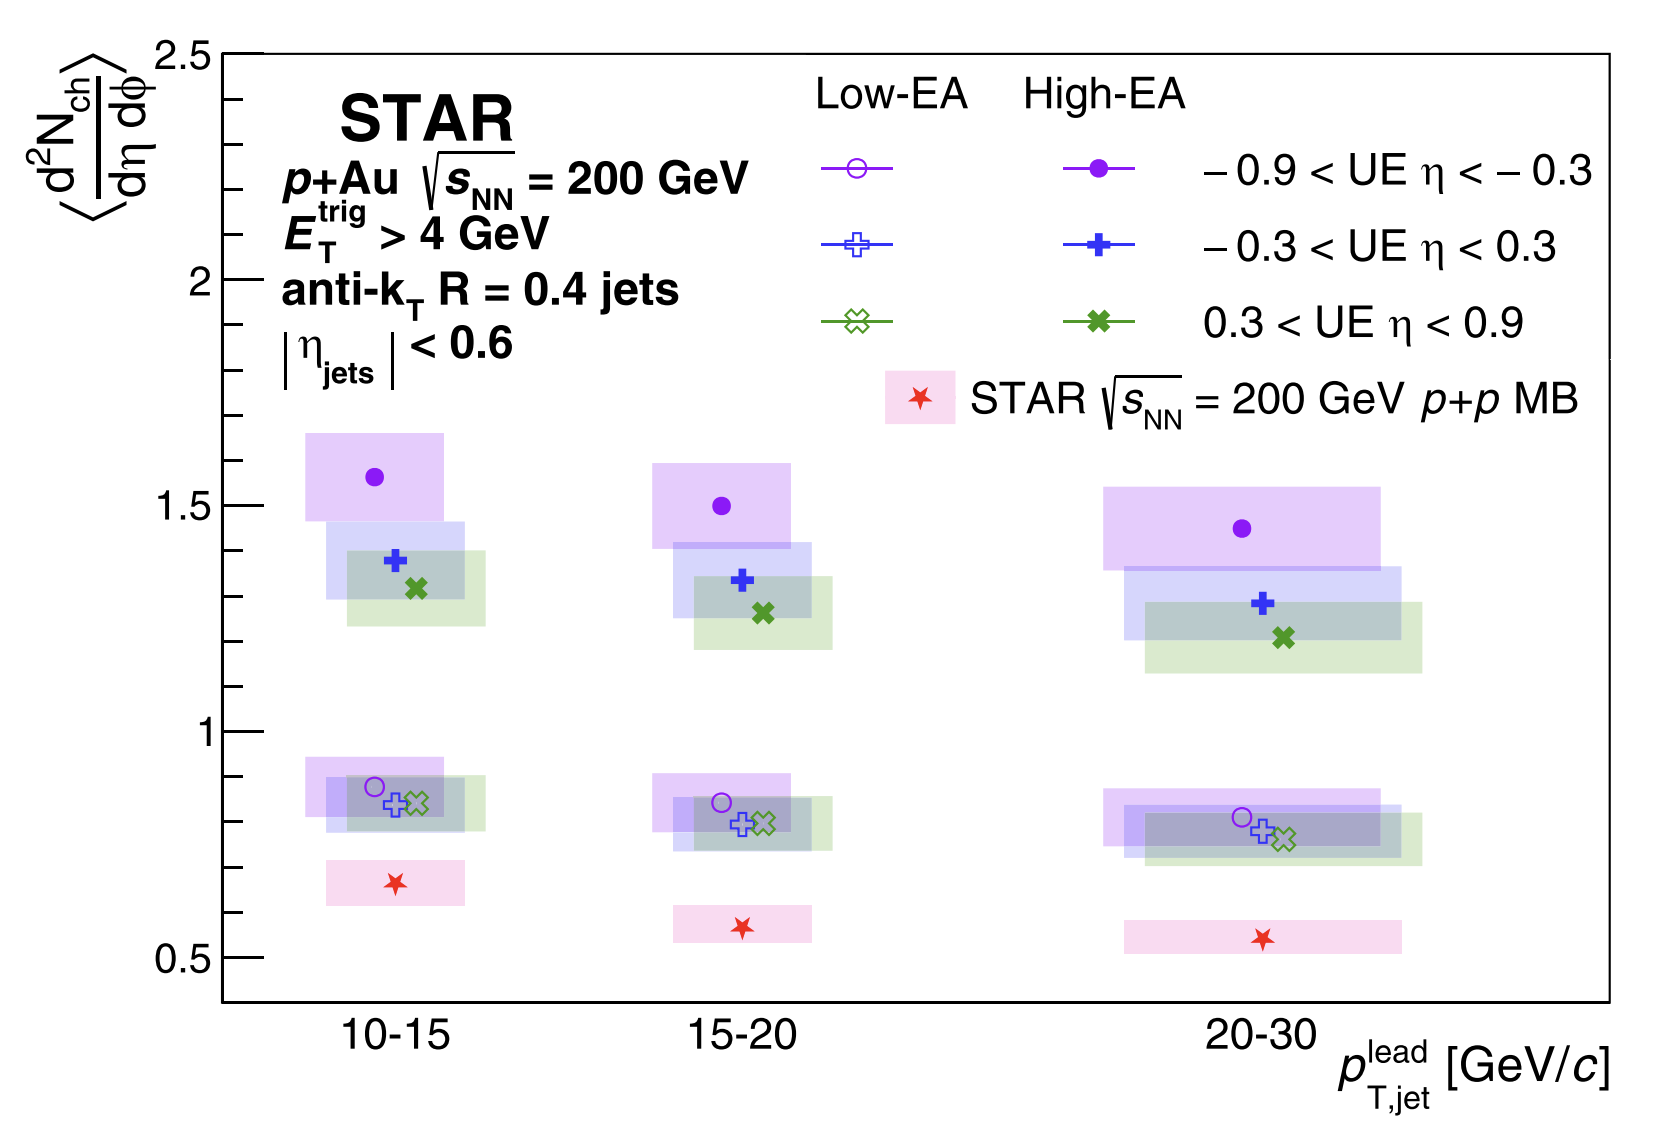
\includegraphics[width=0.7\textwidth]{figures/chapter1/star_ue_in_pAu.png}
    \caption{Underlying event measurements in p+Au collisions at 200 GeV from STAR. Plot shows the underlying event as a function of leading jet pT for dijet events for a selection of events with high- and low-event activity as determined from the forward region. Reproduced from~\cite{star_ue_pAu}.}
    \label{fig:ue_pAu_star}
\end{figure}
\begin{figure}
    \centering
    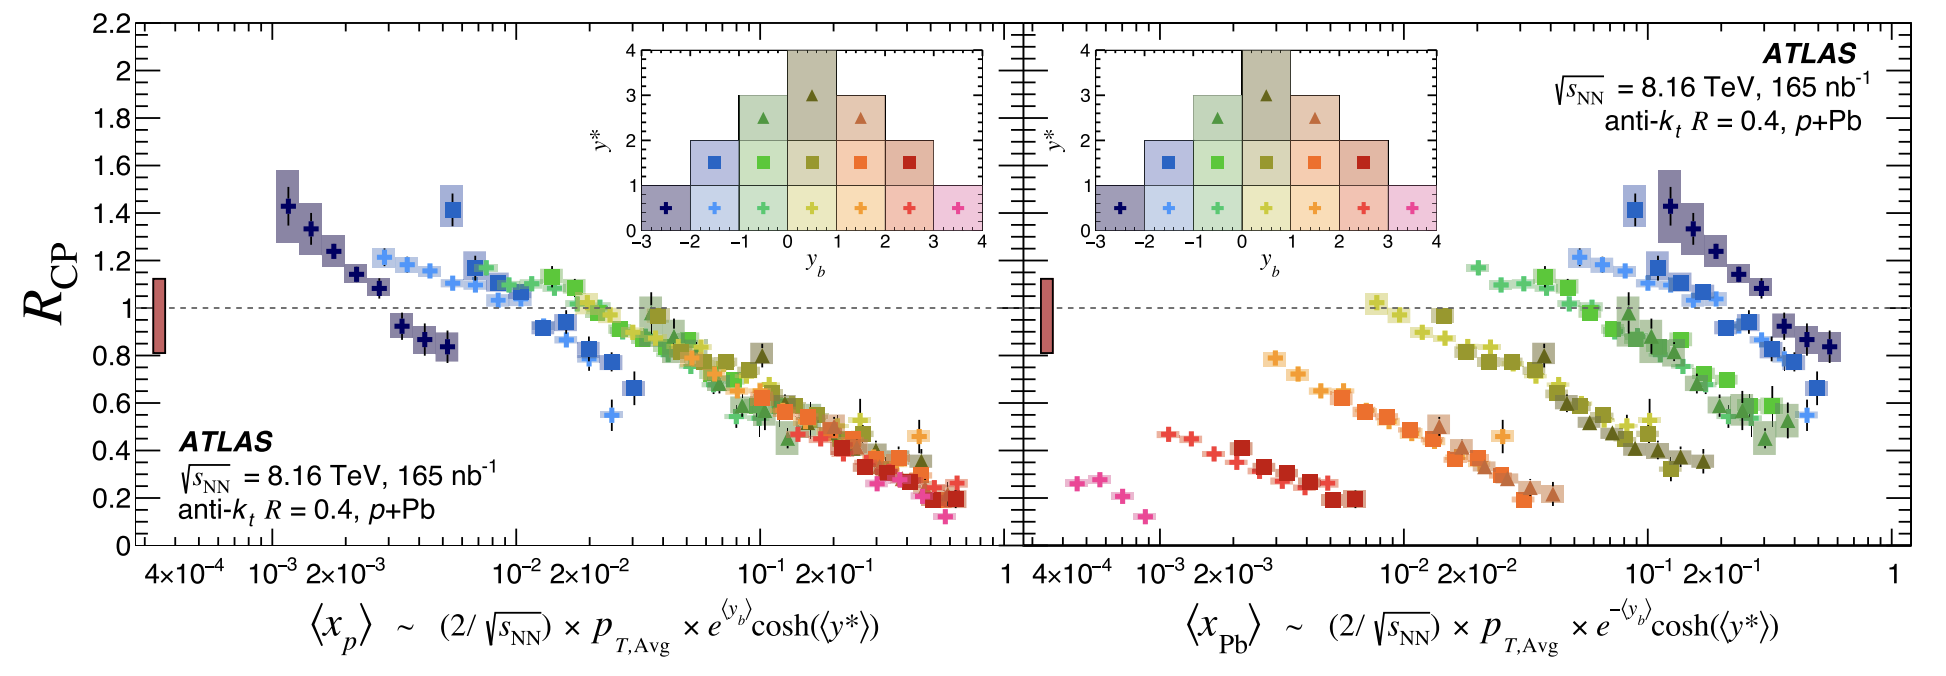
\includegraphics[width=\textwidth]{figures/chapter1/atlas_RpA_dijet.png}
    \caption{Dijet measurements in p+p collisions at 7 TeV from ATLAS. The left plots shows the dijet Rcp as a function of proton parton x, while the right plots shows the dijet Rcp as a function of the lead ion parton x. Reproduced from~\cite{ATLAS:2024dijet_centrality_pPb_816tev}.}
    \label{fig:dijet_pPb_atlas}
\end{figure}
\begin{figure}
    \centering
    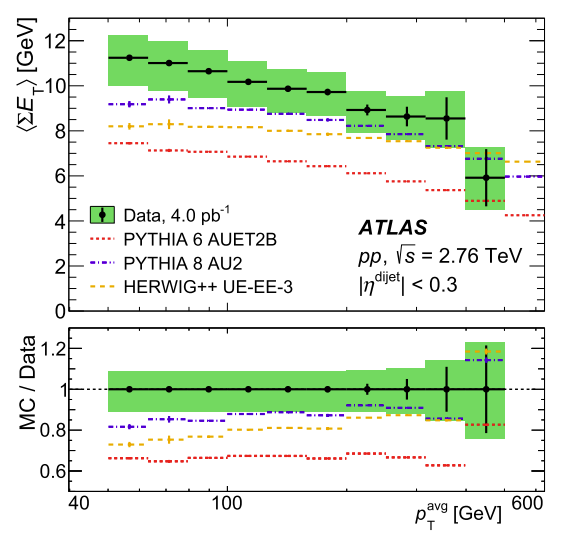
\includegraphics[width=0.7\textwidth]{figures/chapter1/atlas_dijet_pp_EA_vs_pt.png}
    \caption{Underlying event measurements in p+p collisions at 7 TeV from ATLAS. Plot shows the underlying event as a function of leading jet pT for exclusive dijet events for a selection of events with high- and low-event activity as determined from the forward region. Reproduced from~\cite{ATLAS:2016transverse_energy_pp_276tev}.}
    \label{fig:atlas_dijet_pp_EA_vs_pt}
\end{figure}
\begin{figure}
    \centering
    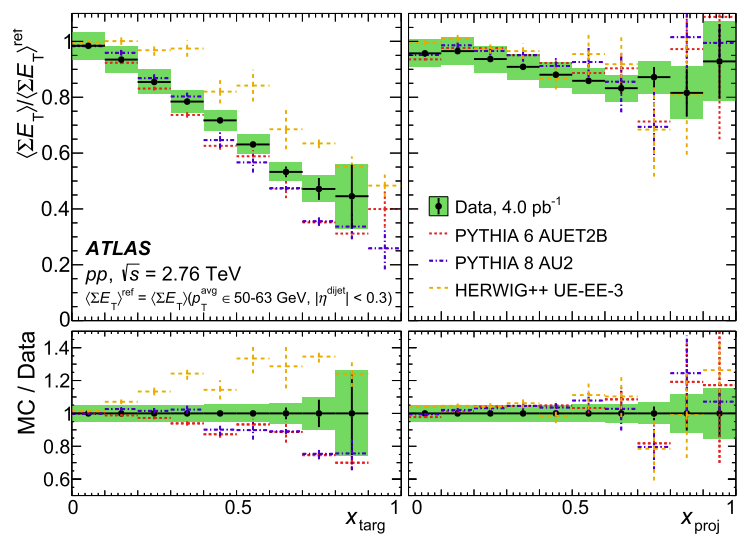
\includegraphics[width=\textwidth]{figures/chapter1/atlas_dijet_pp_EA_vs_x.png}
    \caption{Underlying event measurements in p+p collisions at 7 TeV from ATLAS. Plot shows the underlying event as a function of leading jet pT for exclusive dijet events for a selection of events with high- and low-event activity as determined from the forward region, but plotted as a function of the proton parton x instead of the leading jet pT. Reproduced from~\cite{ATLAS:2016transverse_energy_pp_276tev}.}
    \label{fig:atlas_dijet_pp_EA_vs_x}
\end{figure}

Figure~\ref{fig:unfolded_pt} presents the unfolded underlying event observable, 
$\langle \Sigma E_{T}/\delta\eta\delta\phi \rangle$, as a function of the leading jet transverse momentum for both inclusive jet and dijet event selections. The results are compared to generator-level predictions from \textsc{Pythia8} and \textsc{Herwig7}.

\begin{figure}[htbp]
    \centering
    
\includegraphics[width=0.48\linewidth]{fig/h_result_inclusive.png}
    
\includegraphics[width=0.48\linewidth]{fig/h_result_dijet.png}
    \caption{
    Underlying event transverse energy density, $\langle \Sigma E_{T}/\delta\eta\delta\phi \rangle$, as a function of leading jet $p_{T}$ for inclusive jet (left) and dijet (right) event selections. Data (black points) are shown with statistical uncertainties (bars) and systematic uncertainties (blue bands). The results are compared to generator-level predictions from \textsc{Pythia8} (red line) and \textsc{Herwig7} (green line).
    }
    \label{fig:unfolded_pt}
\end{figure}

A consistent trend is observed in both event selections: the underlying event transverse energy density decreases with increasing leading jet $p_{T}$. While the overall normalization of the measurement is affected by sizable systematic uncertainties, these uncertainties are strongly correlated across jet $p_{T}$ bins. As a result, the shape of the distribution and its dependence on the hard scale are more precisely constrained than the absolute scale. Additionally, the inclusive jet and dijet measurements are in agreement within their uncorrelated uncertainties, indicating that the observed anti-correlation is not significantly sensitive to requiring a dijet event selections at RHIC energies.

The observed decrease of UE activity with increasing jet $p_{T}$ indicates a non-trivial correlation between the hard scattering scale and soft particle production at RHIC energies. In a naive picture of the underlying event, higher-$Q^{2}$ scatterings are expected to be associated with both increased initial- and final-state radiation and a more central overlap of the colliding nucleons, leading to enhanced multiple parton interactions and, therefore, increased UE activity. Instead, we observe that the UE transverse energy density decreases with increasing jet $p_{T}$ indicating an overall energy conservation phenomena which is consistent between inclusive jet and dijet selections and suggests that the interplay between soft and hard processes at RHIC energies is more subtle than a simple scaling of radiation effects with the hard scattering scale.

Comparisons to \textsc{Pythia8} show that the generator reproduces the observed trend. Both \textsc{Pythia8} and \textsc{Herwig} incorporate multiple parton interactions through an impact-parameter-dependent framework and include initial- and final-state radiation tied to the hard scattering scale. However, a key distinction lies in how the interplay between these components is modeled. In \textsc{Pythia8}, multiple parton interactions are interleaved with parton shower evolution in a common $p_T$-ordered sequence, introducing a dynamical and tunable competition between soft and hard processes. This framework allows the relative contributions of MPI and radiation to evolve with the event kinematics, leading to a correlated dependence of UE activity on the leading jet $p_T$.

In contrast, \textsc{Herwig} treats multiple parton interactions and parton shower evolution in a more factorized manner, without an explicit interleaved competition between soft and hard components. As a result, the underlying event activity is more weakly coupled to the hard scattering scale. The sensitivity of the present measurement to the evolution of UE activity with jet $p_T$ therefore provides a discriminating test of these modeling approaches and places important constraints on the description of soft--hard interplay in $p+p$ collisions at RHIC energies.